\chapter{Információs technológiai infrastruktúrák}
\section{A klasszikus IT infrastruktúra}
A klasszikusnak mondott IT infrastruktúrát az írás korábbi részében már bemutattam. Itt most a háromrétegű architektúra egyes rétegeinek skálázását, megbízhatósági szintjének növelésére adott lehetőségeket szeretném bemutatni.
\subsection{Adatbázis réteg}
\todo{Klaszterek, replikák, stb.}
\subsection{Alkalmazás réteg}
\todo{PHP, Java skálázás?}
\subsection{Webkiszolgáló réteg}
\todo{Loadbalancing} 
\section{Felhőalapú infrastruktúrák}
\subsection{Mi is az a ,,számítási felhő''?}

A ,,számítási felhő'' (angolul \foreignlanguage{english}{cloud computing}) egy modell kényelmes, hálózaton keresztül hozzáférhető, konfigurálható számítási erőforrások (pl. hálózat, szerverek, tárhelyek, alkalmazások és szolgáltatások) egy megosztott készletének elérhetőségére, mely erőforrásokat minimális intézkedési erőfeszítéssel vagy szolgáltatói közbenjárással gyorsan rendelkezésre lehet bocsátani \cite{nistsp800-145}.

\todo{Lehet, hogy még finomítani kell a fordításon!}

\begin{comment}
Cloud computing is a model for enabling ubiquitous, convenient, on-demand network access to a shared pool of configurable computing resources (e.g., networks, servers, storage, applications, and services) that can be rapidly provisioned and released with minimal management effort or service provider interaction. 
\end{comment}

Általában hivatkozás szintjén nincsenek elkülönítve az Interneten keresztül szolgáltatott alkalmazások, és a felhő infrastrukturális részét képező hardverek, szoftverek, amelyek ezeket az alkalmazásokat elérhetővé teszik. Ahogy azt \aref{fig:cloud_computing_hu}.~ábrán is szemléltetni próbálom a felhő részét képezi az alkalmazás, szolgáltatás, és a hardver is.

\begin{figure}[h!]
\centering
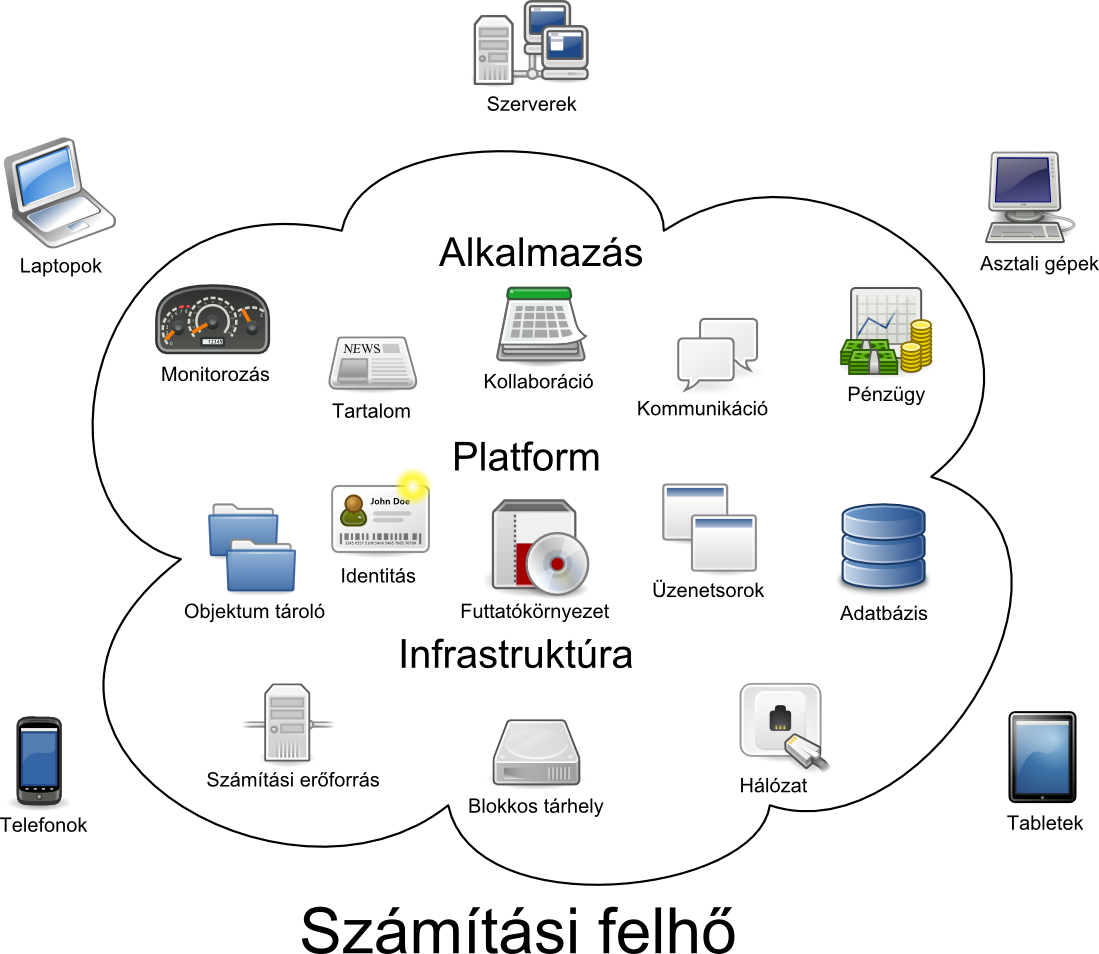
\includegraphics[width=1.0\textwidth]{figures/Cloud_computing_hu.png}
\caption{A számítási felhő (\foreignlanguage{english}{cloud computing}) (Forrás: \href{https://en.wikipedia.org/wiki/File:Cloud\_computing.svg}{Wikipedia})} \label{fig:cloud_computing_hu}
\end{figure}

Mélyebb elemzés során azonban a felhőt rétegekre lehet bontani, amely rétegeket a következő alfejezetben részletezném.

\subsection{A felhő rétegei}

\todo{Ezek lehet inkább szolgáltatás modellek?}

\todo{XaaS service ábrán ne legyen kidomborítva, hogy egymásra épülnek!}

A felhő napjainkban négy architekturális rétegből épül fel, amelyeket alulról fölfelé érdemes megvizsgálni.


\begin{figure}[h!]
\centering
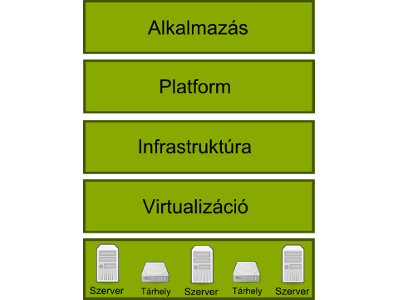
\includegraphics[width=0.25\textwidth]{figures/cloud_retegek.png}
\caption{A számítási felhő rétegei \label{fig:cloud_retegek}}
\end{figure}

\begin{figure}[h!]
\centering
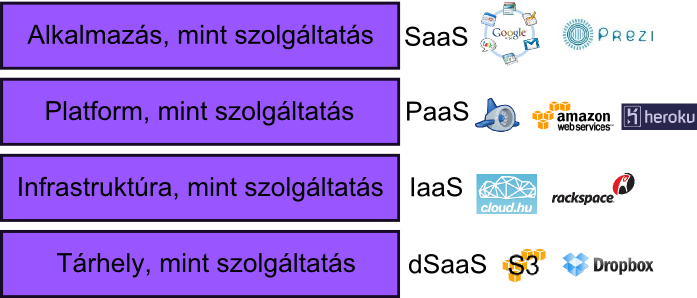
\includegraphics[width=0.5\textwidth]{figures/cloud_service_models.png}
\caption{A számítási felhő szolgáltatási modelljei \label{fig:cloud_service_models}}
\end{figure}
 
\subsubsection{Adattár, mint szolgáltatás (\foreignlanguage{english}{data-Storage-as-a-Service, dSaaS})}
Ezt a réteget \todo{szolgáltatást???} nem minden irodalom szokta említeni, ám én itt mégis külön kezelném, hiszen ez a felhő legalapvetőbb szolgáltatása. Lényege, hogy online tárhelyet biztosít a felhasználóknak. Ilyen szolgáltatást nyújt pl. a \href{http://www.dropbox.com}{Dropbox.com} (főleg személyes felhasználásra, biztonsági mentés, megosztás céljából) vagy az \href{https://aws.amazon.com/s3/}{Amazon S3} (inkább nagy szolgáltatók használják).

A dSaaS oktatási rendszerek esetében sok, nagyméretű adatok esetén lehet előnyös, hiszen nem kell a saját szerverünkön tárolni ezeket, megspórolva ezzel saját adattároló rendszer kialakítását, üzemeltetését. Érdemes megjegyezni, hogy sok adatpéldány esetén is érdemes lehet hasonló szolgáltatás használata, hiszen ebben az esetben az autentikációhoz kötött adatoknál már nem kell a session-öket kezelni, az adatok elérhetőségét megadó URL már tartalmaz egy kódot, csökkentve ezzel a web és alkalmazás szerver terheltségét. 

\todo{dSaaS-ról még valami?}

\todo{Ha a két ábrát össze kellene lőni, ez a legalsó réteg?}

\subsubsection{Infrastuktúra, mint szolgálatás (\foreignlanguage{english}{Infrastructure-as-a-Service, IaaS})}

Az infrastruktúra, mint szolgáltatás az előfizető számára rendelkezésre bocsájt olyan feldolgozási, tárhely, hálózati és egyéb alapvető számítási erőforrásokat, ahol az előfizető képes telepíteni és futtatni tetszőleges szoftvert, amely szoftver magába foglalhatja magát az operációs rendszert és egyéb alkalmazásokat is. Az előfizető nem kezeli a szolgáltatás alapjául szolgáló infrastruktúrát, de irányítása alá tartozik az operációs rendszer, a tárhely és a telepített alkalmazások; esetleg korlátozottan hálózati komponensek (pl. tűzfalak).\cite{nistsp800-145}

IaaS is the leasing of infrastructure (computing resources and storage) as a service. This means not only virtualized computers with guaranteed processing power but reserved bandwidth for storage and Internet access. In essence, it's the capability of leasing a computer or data center with specific quality-of-service constraints that has the ability to execute an arbitrary operating system and software.\cite{ccwlinux}





\todo{IaaS}
\subsubsection{Platform, mint szolgáltatás (\foreignlanguage{english}{Platform-as-a-Service, PaaS})}

\foreignlanguage{english}{''The capability provided to the consumer is to deploy onto the cloud infrastructure consumer-created or acquired applications created using programming languages, libraries, services, and tools supported by the provider. The consumer does not manage or control the underlying cloud infrastructure including network, servers, operating systems, or storage, but has control over the deployed applications and possibly configuration settings for the application-hosting environment. This capability does not necessarily preclude the use of compatible programming languages, libraries, services, and tools from other sources.''}\cite{nistsp800-145}

\todo{PaaS}
\subsubsection{Szoftver, mint szolgáltatás (\foreignlanguage{english}{Software-as-a-Service,SaaS})}

\foreignlanguage{english}{''The capability provided to the consumer is to use the provider’s applications running on a cloud infrastructure. A cloud infrastructure is the collection of hardware and software that enables the five essential characteristics of cloud computing. The cloud infrastructure can be viewed as containing both a physical layer and an abstraction layer. The physical layer consists of the hardware resources that are necessary to support the cloud services being provided, and typically includes server, storage and network components. The abstraction layer consists of the software deployed across the physical layer, which manifests the essential cloud characteristics.  Conceptually the abstraction layer sits above the physical layer. The applications are accessible from various client devices through either a thin client interface, such as a web browser (e.g., web-based email), or a program interface. The consumer does not manage or control the underlying cloud infrastructure including network, servers, operating systems, storage, or even individual application capabilities, with the possible exception of limited user-specific application configuration settings.''}\cite{nistsp800-145}

\todo{SaaS}

\todo{Deployment Models}
